
\section{Rotational Matrix for $\mathbb{R}^2$}
The Rotational Matrix for rotating a coordinate system in 2 dimensions is commonly stated as
\[
R(\theta) = \left[ \begin{matrix}
\cos(\theta) & -\sin(\theta) \\
sin(\theta) &  \cos(\theta) 
\end{matrix}\right]
\]
Where it is applied to a Cartesian cordinate system as
\[
\left[ \begin{matrix}
\cos(\theta) & -\sin(\theta) \\
\sin(\theta) &  \cos(\theta) 
\end{matrix}\right] 
\left[ \begin{matrix}
x' \\
y'
\end{matrix} \right] =
\left[ \begin{matrix}
x \\
y
\end{matrix} \right]
\]
where x' and y' are the rotated coordinates.

\subsection{Derivation}
A positional vector denotes a point (x,y) in the Cartesian Coordinate System.  This positional point has an angle of \(\theta\) and a magnitude of \(\sqrt{x^2 + y^2}\) \\
\\
\begin{center}

\includegraphics[width=8cm]{Linear_Algebra/rotational_matrix_diag1}
\end{center}

Now rotate the entire coordinate system by an angle \(\theta\)\\
\begin{center}
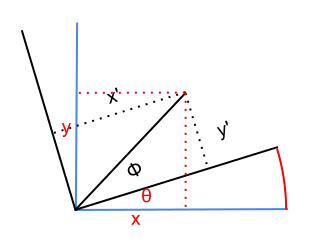
\includegraphics[width=8cm]{Linear_Algebra/rotational_matrix_diag2}
\end{center}

\begin{align*}
x &= \sqrt{(x')^2 + (y')^2}\cos(\phi + \theta) \\
y &= \sqrt{(x')^2 + (y')^2}\sin(\phi + \theta)\\
\\
x &= \sqrt{(x')^2 + (y')^2}(\cos(\phi)\cos(\theta) - \sin(\phi)\sin(\theta) ) \\
y &= \sqrt{(x')^2 + (y')^2}(\sin(\phi)\cos(\theta) + cos(\phi)sin(\theta) )\\
\\
x &= x'\frac{\sqrt{(x')^2 + (y')^2}}{x'}(\cos(\phi)\cos(\theta) - \sin(\phi)\sin(\theta) ) \\
y &= y'\frac{\sqrt{(x')^2 + (y')^2}}{y'}(\sin(\phi)\cos(\theta) + \cos(\phi)\sin(\theta) )\\
\\
x &= x'\frac{1}{\cos(\phi)}(\cos(\phi)\cos(\theta) - \sin(\phi)\sin(\theta) ) \\
y &= y'\frac{1}{\sin(\phi)}(\sin(\phi)\cos(\theta) + \cos(\phi)\sin(\theta) )\\
\\
x &= x'(\cos(\theta) - \tan(\phi)\sin(\theta) ) \\
y &= y'(\cos(\theta) + \cot(\phi)sin(\theta) ) \\
\\
x &= x'(\cos(\theta) - \frac{y'}{x'}\sin(\theta) ) \\
y &= y'(\cos(\theta) + \frac{x'}{y'}\sin(\theta) ) \\
\\
x &= x'\cos(\theta) - y'\sin(\theta) \\
y &= y'\cos(\theta) + x'\sin(\theta)  \\
\\
\left[
\begin{matrix}
x\\
y
\end{matrix}
\right] &=
\left[ \begin{matrix}
\cos(\theta) & -\sin(\theta) \\
\sin(\theta) &  \cos(\theta) 
\end{matrix}\right] 
\left[ \begin{matrix}
x' \\
y'
\end{matrix} \right]
\end{align*}

\section{Rotational Matrix for $\mathbb{R}^3$}
The Rotational Matrices in 3 dimensions can be stated as
\[
R_z(\theta) = \left[ \begin{matrix}
\cos(\theta) & -\sin(\theta) & 0\\
\sin(\theta) &  \cos(\theta) & 0\\
0 & 0 & 1 
\end{matrix}\right]
\]
For a rotation about the z-axis\\
\[
R_y(\theta) = \left[ \begin{matrix}
\cos(\theta) &  0 &-\sin(\theta) \\
0 & 1 & 0 \\
\sin(\theta) &  0 &\cos(\theta)\\
\end{matrix}\right]
\]
For a rotation about the y-axis
\[
R_x(\theta) = \left[ \begin{matrix}
1 & 0 & 0\\
0 & \cos(\theta) & -\sin(\theta) \\
0 & \sin(\theta) &  \cos(\theta) \\
\end{matrix}\right]
\]
For a rotation about the x-axis
\\
\subsection{Explanation}
It's almost obvious that from \\
\[
\left[ \begin{matrix}
\cos(\theta) & -\sin(\theta) \\
\sin(\theta) &  \cos(\theta) 
\end{matrix}\right] 
\left[ \begin{matrix}
x' \\
y'
\end{matrix} \right] =
\left[ \begin{matrix}
x \\
y
\end{matrix} \right]
\]
We can extend it to\\
\[
\left[ \begin{matrix}
\cos(\theta) & -\sin(\theta) & 0\\
\sin(\theta) &  \cos(\theta) & 0\\
0 & 0 & 1
\end{matrix}\right] 
\left[ \begin{matrix}
x' \\
y' \\
z'
\end{matrix} \right] =
\left[ \begin{matrix}
x \\
y \\
z
\end{matrix} \right]
\]
And this could be exteneded beyond 3 dimensions.\\
\\
It is important to note that the order of these rotations is important
\[R_zR_yR_xX \ne R_xR_yR_zX\]
\\
To demonstrate this take a Rubik's Cube and orient it with the white side facing up, blue facing front, orange facing right (yellow down, red left, green back).  This is your starting position. \\
\\
Now rotate:\\
clockwise about the front, clockwise about the top, clockwise about the right.\\
\\
This is not the result if you do the reverse order:\\
clockwise about the right, clockwise about the top, clockwise about the front\\
\\
This is because matrix multiplication is not commutative.


